\chapter{Diseño e implementación}
\label{Chapter3}

\definecolor{mygreen}{rgb}{0,0.6,0}
\definecolor{mygray}{rgb}{0.5,0.5,0.5}
\definecolor{mymauve}{rgb}{0.58,0,0.82}

\lstset{ %
  backgroundcolor=\color{white},   % choose the background color; you must add \usepackage{color} or \usepackage{xcolor}
  basicstyle=\footnotesize,        % the size of the fonts that are used for the code
  breakatwhitespace=false,         % sets if automatic breaks should only happen at whitespace
  breaklines=true,                 % sets automatic line breaking
  captionpos=b,                    % sets the caption-position to bottom
  commentstyle=\color{mygreen},    % comment style
  deletekeywords={...},            % if you want to delete keywords from the given language
  %escapeinside={\%*}{*)},          % if you want to add LaTeX within your code
  %extendedchars=true,              % lets you use non-ASCII characters; for 8-bits encodings only, does not work with UTF-8
  %frame=single,	                % adds a frame around the code
  keepspaces=true,                 % keeps spaces in text, useful for keeping indentation of code (possibly needs columns=flexible)
  keywordstyle=\color{blue},       % keyword style
  language=[ANSI]C,                % the language of the code
  %otherkeywords={*,...},           % if you want to add more keywords to the set
  numbers=left,                    % where to put the line-numbers; possible values are (none, left, right)
  numbersep=5pt,                   % how far the line-numbers are from the code
  numberstyle=\tiny\color{mygray}, % the style that is used for the line-numbers
  rulecolor=\color{black},         % if not set, the frame-color may be changed on line-breaks within not-black text (e.g. comments (green here))
  showspaces=false,                % show spaces everywhere adding particular underscores; it overrides 'showstringspaces'
  showstringspaces=false,          % underline spaces within strings only
  showtabs=false,                  % show tabs within strings adding particular underscores
  stepnumber=1,                    % the step between two line-numbers. If it's 1, each line will be numbered
  stringstyle=\color{mymauve},     % string literal style
  tabsize=2,	                   % sets default tabsize to 2 spaces
  title=\lstname,                  % show the filename of files included with \lstinputlisting; also try caption instead of title
  morecomment=[s]{/*}{*/}
}

Este capítulo detalla la generación de contenido original del trabajo.
Se explica su diseño y producción.

\section{Autoevaluación del dispositivo bajo prueba}
\label{sec:autoevaluacion}

La construcción del \emph{firmware} de autoevaluación del dispositivo bajo prueba requirió superar las siguientes etapas:
\begin{itemize}
    \item Configuración de las señales de reloj del dispositivo bajo prueba.
    \item Selección y configuración de los periféricos del dispositivo bajo prueba.
    \item Selección y configuración de los terminales externos del dispositivo bajo prueba.
    \item Implementación de las estrategias de validación de periféricos.
    \item Integración de una secuencia de validación y reporte.
\end{itemize}

Para configurar las frecuencias de reloj se buscó obtener 150 MHz para suministrar al \emph{Master CAN Bus}.
Con esta condición satisfecha, se pudo configurar las frecuencias de reloj del resto de los periféricos.
En la figura \ref{fig:clock} se puede observar la utilización del \emph{Programmable Clock Controller} número cinco.

\begin{figure}[htbp]
	\centering
	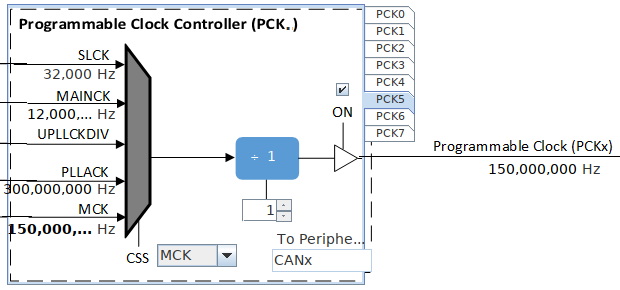
\includegraphics[width=\textwidth]{./Figures/Clock.png}
    \caption{Diagrama de configuración de las señales de reloj.}
	\label{fig:clock}
\end{figure}

El siguiente paso en la etapa de diseño fue la selección de las instancias de los periféricos del integrado.
Es posible que dos periféricos compartan parte del circuito interno o terminales del encapsulado.
Esta situación puede generar una disminución en las funcionalidades o una total incompatibilidad.
Finalmente, se seleccionaron instancias completamente disjuntas.

Luego de seleccionar las instancias de los periféricos, se configuraron para realizar un \emph{loopback}.
La configuración se realizó de la siguiente manera:

\begin{itemize}
    \item \emph{CAN}: se utilizó el \emph{MCAN1} con una configuración de \emph{loopback} interna, como se puede ver en la figura \ref{fig:canloopback}.
    \item \emph{PIO}: se configuraron dos terminales del dispositivo bajo prueba.
        El primero como salida sin \emph{latch} y el segundo como entrada sin circuito anti rebote.
    \item \emph{SPI}: la configuración elegida fue por defecto ya que el \emph{loopback} se logró conectando \emph{TX} y \emph{RX} con un cable.
    \item \emph{UART}: se configuró el periférico con una velocidad de 9600 baudios, 8 bits de datos y sin bits de paridad.
    \item \emph{Watchdog}: el disparo se configuró con un contador en 4095 cuentas.
        Este valor se estimó entre dos y cinco ejecuciones del \emph{loop} principal.
\end{itemize}

\begin{figure}[htbp]
	\centering
	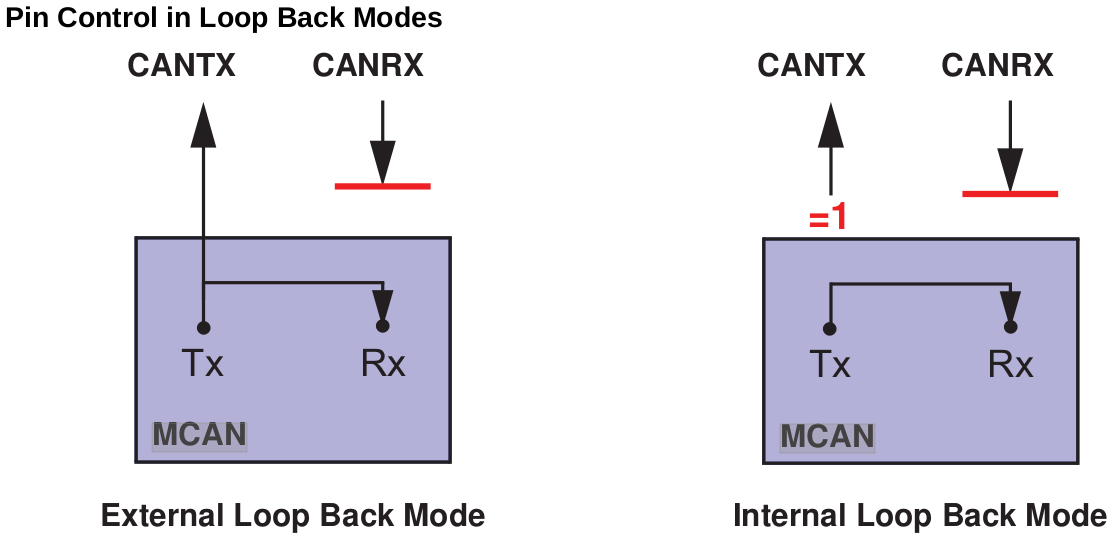
\includegraphics[width=0.8\textwidth]{./Figures/canloopback.png}
    \caption{Diagrama de \emph{loopback} del periférico \emph{CAN}\protect\footnotemark.}
	\label{fig:canloopback}
\end{figure}

\footnotetext{Imagen tomada de la hoja de datos del dispositivo bajo prueba \citep{ARTICLE:dutdatasheet}.}

Como se puede ver en la figura \ref{fig:labo}, se priorizaron los \emph{loopbacks} físicos externos.
Cuando esta estrategia no fue posible, se optó por internos provistos por el fabricante.
Finalmente, en los casos que las dos primeras opciones fueron imposibles, se utilizó una estrategia de \emph{software}.
En la tabla \ref{tab:perifericos} se puede ver un resumen de las estrategias aplicadas.

\begin{table}[h]
	\centering
	\caption[Estrategias de depuración]{Comparación entre estrategias de depuración}

	\begin{tabular}{l c c}    
		\toprule
        \textbf{Periférico} & \textbf{Validación}       & \textbf{Detección en un ciclo}\\
		\midrule
		CAN                 & Loopback interno          & Si\\		
		PIO                 & Loopback externo          & No\\
		SPI                 & Loopback externo          & Si\\
		UART                & Lógica en firmware        & No\\
		Watchdog            & Lógica en inyector        & No\\
		\bottomrule
		\hline
	\end{tabular}
	\label{tab:perifericos}
\end{table}

\begin{figure}[htbp]
	\centering
	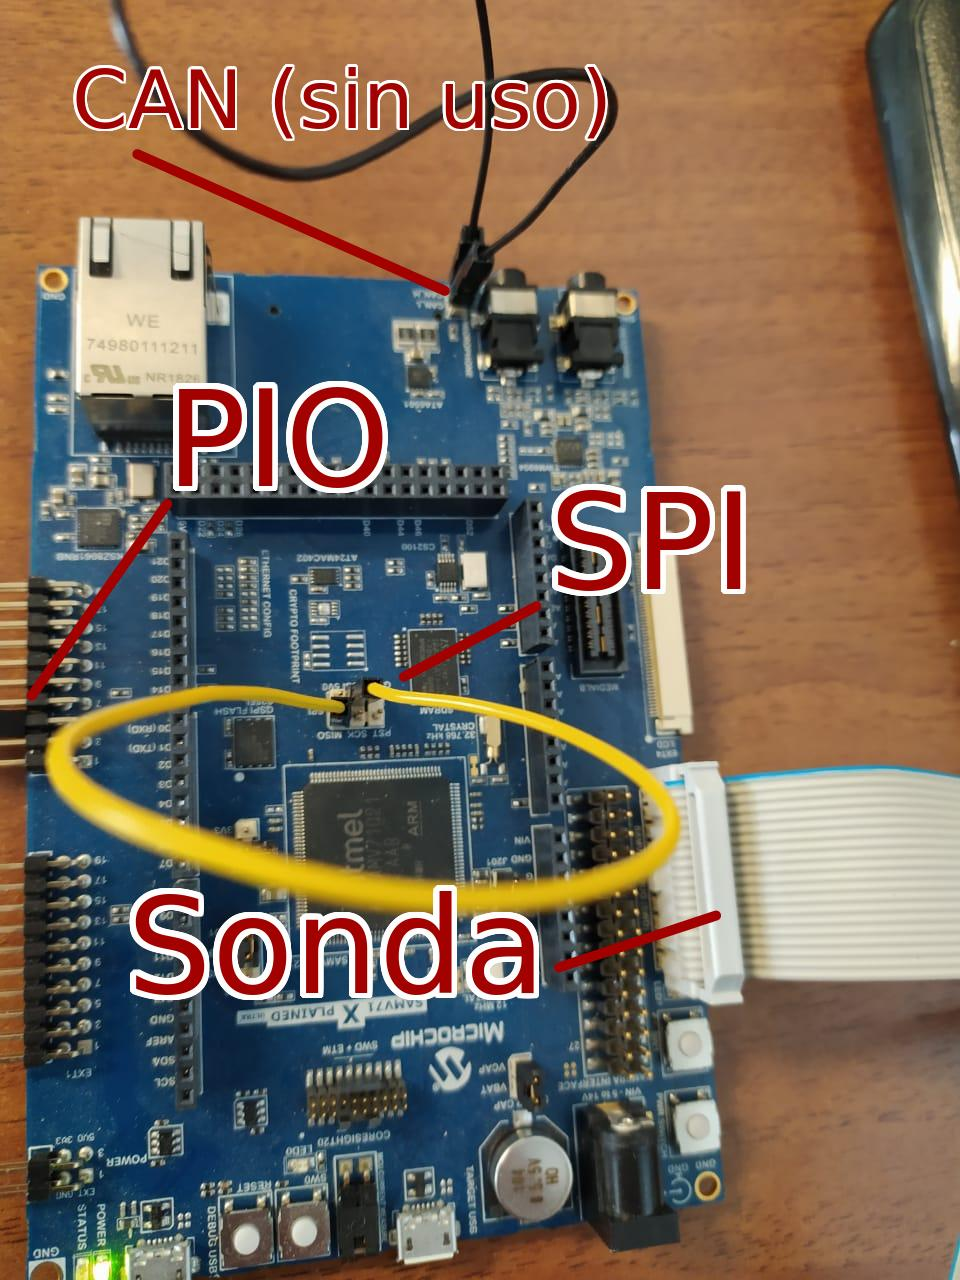
\includegraphics[width=\textwidth]{./Figures/labo.jpeg}
    \caption{Fotografía del dispositivo bajo prueba.}
	\label{fig:labo}
\end{figure}

Una vez configurados los componentes de \emph{hardware} del dispositivo bajo prueba; se procedió a diseñar el \emph{firmware}.
Se comenzó con la estructura que define los reportes de estado del dispositivo bajo prueba.
Los reportes están formados por 2 bytes, el primero es el carácter ``F'' y marca el inicio del reporte mientras que el segundo byte lleva la información del estado de los periféricos.
En el código \ref{cod:structs} se puede ver la implementación del segundo byte del reporte.

\begin{lstlisting}[language=C,label=cod:structs,caption=Definición de la estructura de reportes.]  % Start your code-block

#define BIT 1

struct status_bitfield_t
{
    uint8_t CAN:BIT;
    uint8_t SPI:BIT;
    uint8_t PIO:BIT;
    uint8_t WATCHDOG:BIT;
}__attribute__((packed));

typedef union
{
    struct status_bitfield_t status_of;
    uint8_t packed;
}report_t;

\end{lstlisting}

En el código \ref{cod:loop} se puede observar la implementación del lazo principal.
Es importante notar que en la línea 10 se utilizó la \emph{union} para transformar el reporte en caracteres legibles para una persona.
En la figura \ref{fig:firmwareflow} se puede observar el flujo completo del programa.

\begin{lstlisting}[language=C,label=cod:loop,caption=Lazo principal del \emph{firmware} de autoevaluación.]  % Start your code-block

while ( true )
{
    SYS_Tasks ( );
    report.status_of.CAN = validate_CAN();
    report.status_of.PIO = validate_PIO();
    report.status_of.SPI = validate_SPI();
    report.status_of.WATCHDOG = NORMAL;
    
    buffer[FRAME_START] = 'F';
    buffer[FLAGS_INDEX] = report.packed + 'A';
    USART1_Write(&buffer[0], FRAME_SIZE);
    
    WDT_Clear();
}

\end{lstlisting}

\begin{figure}[htbp]
	\centering
	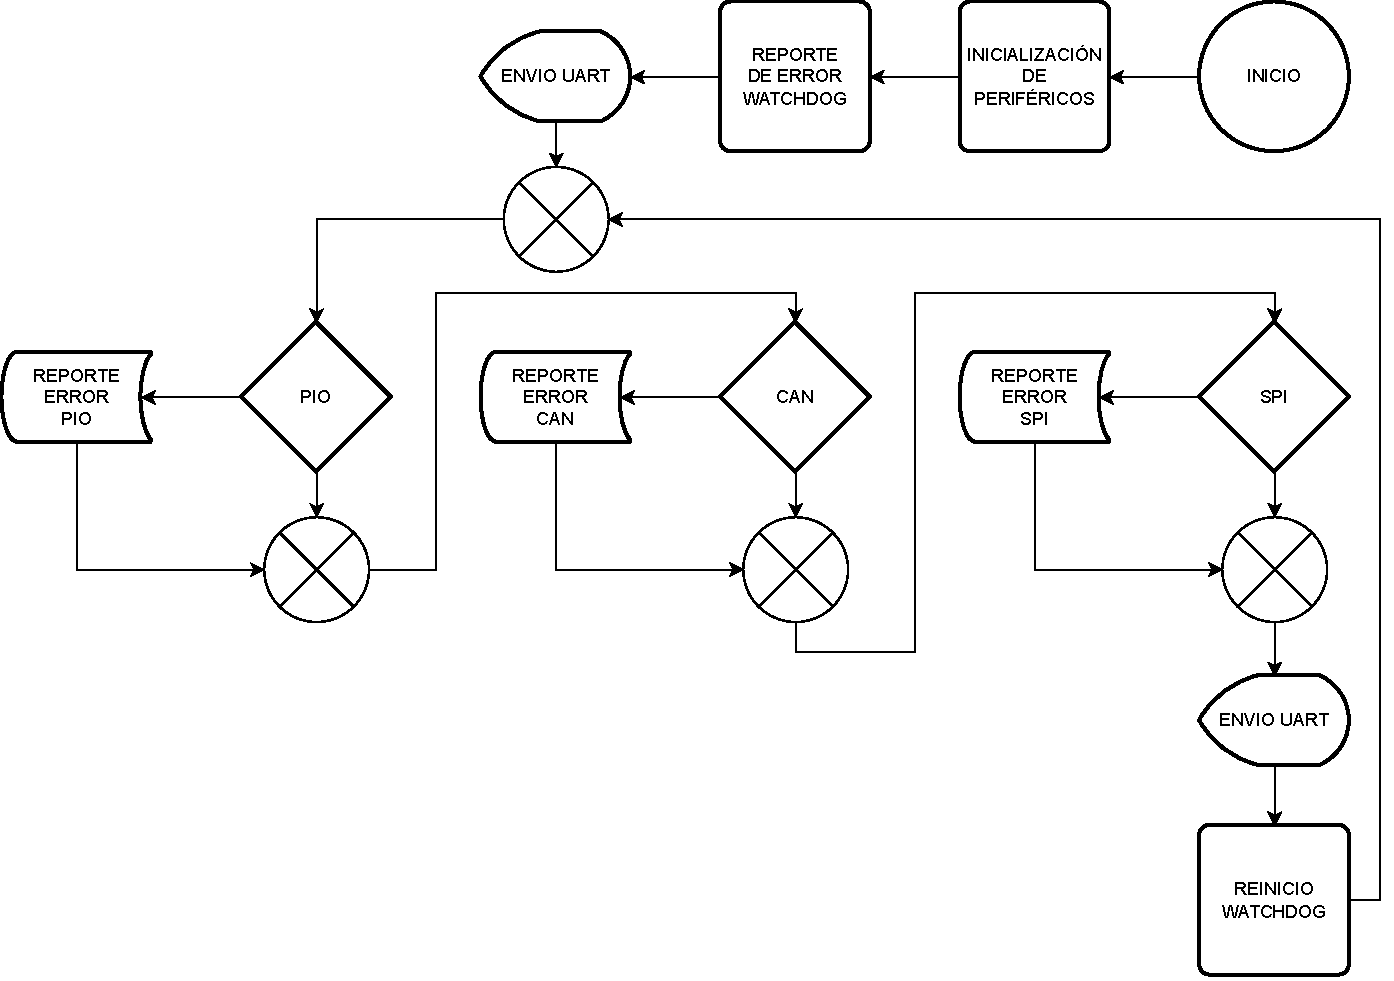
\includegraphics[width=\textwidth]{./Figures/firmwareflow.pdf}
    \caption{Flujo del \emph{firmware} de autoevaluación.}
	\label{fig:firmwareflow}
\end{figure}

\newpage

\section{Interfaz de programación de aplicaciones}
\label{sec:api}

% técnica RAII
% conexión como recurso
La interfaz de programación de aplicaciones tiene la función de abstraer al inyector de errores del servidor \emph{OCD}.
Esto se logró con los siguientes patrones de diseño:

\begin{itemize}
    \item Programación orientada a objetos \emph{(OOP)}: este patrón de diseño se basa en agrupar en una unidad lógica las funcionalidades y estados que tengan un alto grado de acoplamiento.
        Esto significa que la funciones que tienen efectos colaterales junto a los datos mutados se encapsulan dentro de una construcción denominada objeto.
        Entonces, el principal objetivo de un objeto es contener dentro suyo los efectos colaterales.
        Además, el lenguaje de programación \emph{Python 3} permite, a través de una \emph{class}, modelar un tipo de dato para instanciar a un objeto.
        Finalmente, este patrón se utilizó para contener las funciones de lectura y escritura de registros y memorias.
    \item \emph{Resource Acquisition Is Initialization (RAII)}: este patrón de diseño consiste en modelar el ciclo de vida de un recurso con la implementación de un objeto.
        Un recurso es todo aquello que requiera mantenimiento luego de su uso, como por ejemplo: liberar memoria, cerrar una conexión o unir dos hilos de un programa.
        Esto se logra al adquirir un recurso cuando se invoca el constructor de una \emph{class}, por ejemplo, la conexión con la sonda de depuración se realiza durante la instanciación de un objeto llamado conexión.
        Luego, cuando se desea cerrar la conexión se invoca al destructor del objeto.
        Dentro de esta función se encuentra el código para cerrar de forma ordenada la conexión con la sonda y el dispositivo bajo prueba.
        Finalmente, este patrón de diseño hace que el programa maneje de forma robusta los recursos ya que está garantizada la ejecución de los destructores.
\end{itemize}

En el código \ref{cod:halted} se puede observar un ejemplo de \emph{RAII} donde se maneja como recurso la detención del núcleo del dispositivo bajo prueba.
Esto permite que frente a una excepción del proceso que esté utilizando la interfaz de programación de aplicaciones, el núcleo pueda continuar operando.
Finalmente, se posibilita recuperar el proceso sin tener que reiniciar el dispositivo bajo prueba.

\begin{lstlisting}[language=Python,label=cod:halted,caption=Ejemplo de \emph{Resource Acquisition Is Initialization (RAII)}.]  % Start your code-block

class Halted():
    def __init__(self, target):
        self.target = target

    def __enter__(self):
        self.target.halt()

    def __exit__(self, exc_type, exc_val, traceback):
        self.target.resume()

\end{lstlisting}

Los patrones de diseño utilizados permiten escribir funciones expresivas y robustas.
Como se puede ver en el código \ref{cod:haltedexample}, es fácil comprender lo que sucede.
En la línea 2 se detiene el núcleo y en la línea 3 se lee una posición de memoria.
Luego, en la línea 4 el núcleo reanuda su funcionamiento y finalmente, se retorna el valor leído.

\newpage

\begin{lstlisting}[language=Python,label=cod:haltedexample,caption=Ejemplo de uso de \emph{RAII}.]  % Start your code-block

def readMemory(self, addr: int):
    with Halted(self.target):
        val = self.target.read_memory(addr)
    return val

\end{lstlisting}

En la tabla \ref{tab:funcionalidades} se puede observar un resumen de las funcionalidades y sus estrategias de abstracción.

\begin{table}[h]
	\centering
	\caption[Funcionalidades abstraidas]{Funcionalidades abstraídas}

	\begin{tabular}{l c c}    
		\toprule
        \textbf{Funcionalidad}     & \textbf{Patrón de diseño} & \textbf{Acceso}\\
		\midrule
		Conexión al integrado      & RAII                      & Público\\		
		Detener el núcleo          & RAII                      & Privado\\
		Registros CORE: read/write & OOP                       & Público\\
		Memoria SDRAM: read/write  & OOP                       & Público\\
		\bottomrule
		\hline
	\end{tabular}
	\label{tab:funcionalidades}
\end{table}

Finalmente, se logró abstraer el ciclo de vida de la sesión de depuración que se muestra en la figura \ref{fig:debugsession}.

\begin{figure}[htbp]
	\centering
	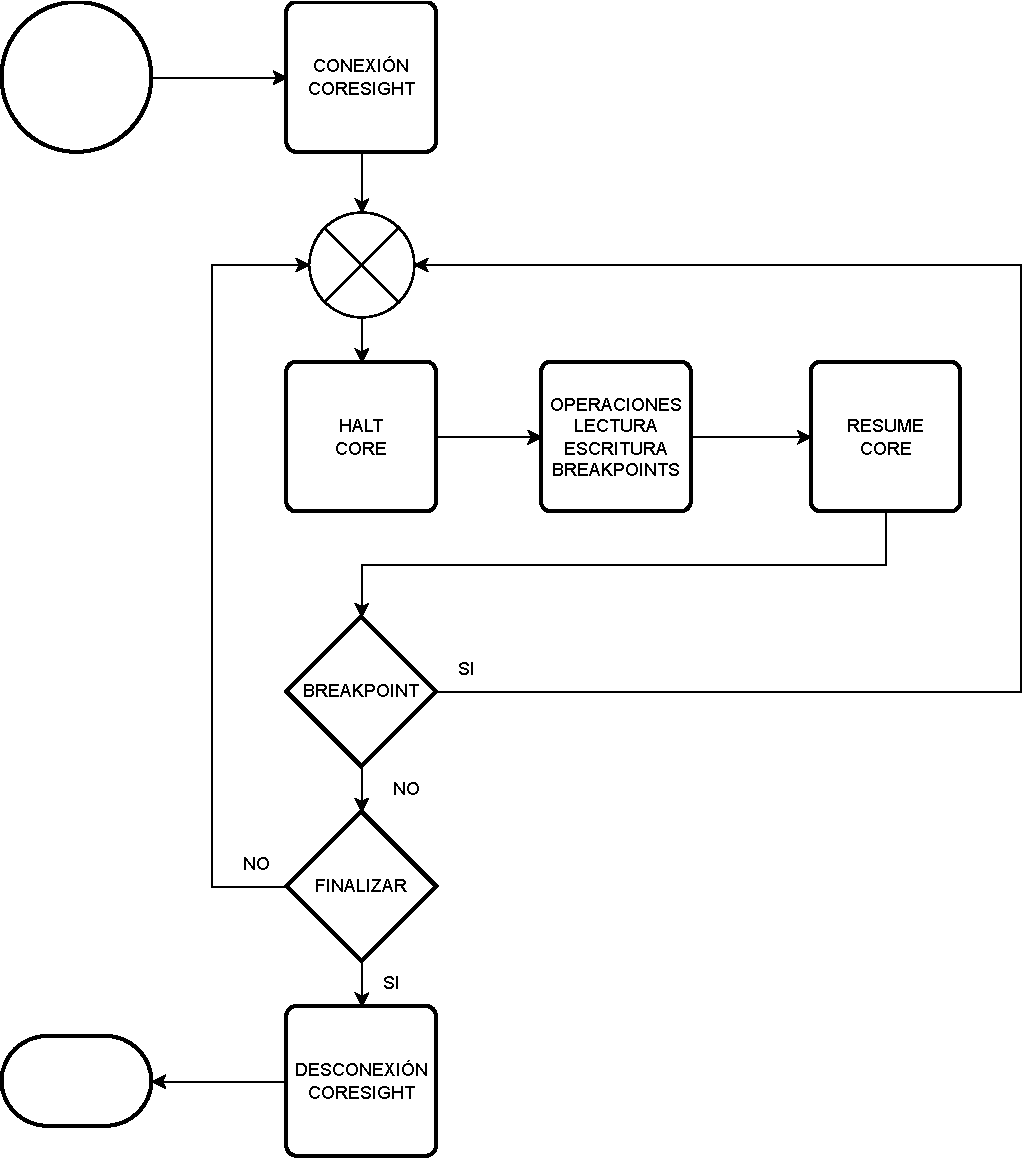
\includegraphics[width=0.9\textwidth]{./Figures/debugsession.pdf}
    \caption{Flujo de una sesión de depuración.}
	\label{fig:debugsession}
\end{figure}

\section{Sistema de inyección de \emph{soft-errors}}
\label{sec:sise}

Una vez lograda la interfaz de programación de aplicaciones explicada en la sección \ref{sec:api}, se pudo construir el inyector por consola de comandos.
Para lograr que el usuario utilice el programa se creó un sistema de archivo de configuración y un cliente de terminal en texto plano.
El archivo de configuración se genera en formato \emph{YAML} y se encarga de:

\begin{itemize}
    \item Definir si el controlador de ensayos debe recoger los reportes del dispositivo bajo prueba.
    \item Configurar el puerto serie del ordenador.
    \item Definir la simulación:
        \begin{itemize}
            \item El tipo de distribución para usar en el planificador de ensayos.
            \item La tasa de inyección de errores.
            \item La duración del tiempo de exposición en un registro o posición de memoria.
            \item La secuencia de exposición de los registros.
        \end{itemize}
\end{itemize}

% Configuración

En el código \ref{cod:yaml} se puede observar un archivo de configuración.
En particular, la configuración que el sistema ofrece como ejemplo al usuario.
Es importante notar que no se hace referencia a la sesión de depuración.
Finalmente, el ensayo se expresa en términos de parámetros de radiación.

Para facilitar la tarea del usuario, una vez instalado el sistema no es necesario trabajar en una carpeta en particular.
El inyector se puede invocar desde cualquier sitio donde el intérprete de Python 3 tenga permisos de ejecución.
El operador puede entonces crear una carpeta del ensayo.
Luego, crear un archivo de configuración y lanzar desde allí mismo la secuencia de inyecciones.
Finalmente, el sistema genera el reporte correspondiente en esa ruta.

\begin{lstlisting}[language=Python,label=cod:yaml,caption=Ejemplo de configuración de ensayo.]  % Start your code-block

# Perfil determina el tipo de ensayo a realizar
# 'simulador' solo genera inyecciones mientras
# que 'evaluador' recoge y procesa los
# reportes del DUT.
Perfil: 'simulador'

# Interfaz define el puerto serie donde se
# conecto el DUT.
Interfaz:
  puerto: '/dev/ttyACM0'
  baudios: 9600

# Simulacion define la forma de inyectar errores
Simulacion:
  distribucion: 'Poisson'
  tasa: 0.5
  duracion: 5
  registros: 'secuencial'

\end{lstlisting}

% Consola

La interfaz por consola se logró al utilizar el \emph{standar input} y el \emph{standar output} del proceso padre.
En el caso de una sesión iniciada por un humano, el emulador de terminal del sistema.
En una primera iteración de la consola se realizó una interfaz ASCII con la biblioteca \emph{curses}.
Sin embargo, el cliente prefirió una interfaz por texto plano para facilitar el \emph{parsing} de un sistema de integración continua.
En particular, el módulo de \emph{CI/CD} de \emph{Gitlab}.

El usuario invoca el programa al ejecutar el comando \texttt{sise}.
Luego la consola responde con la leyenda \texttt{Ingrese el archivo de configuración > }.
Se escribe la ruta y nombre del archivo a utilizar y el sistema lanza el ensayo.
El reporte generado se persiste en la carpeta donde se inició el programa.

% Planificador de ensayos

Con la información suministrada por el archivo de configuración y la consola, se puede iniciar el planificador de ensayos.
Este módulo tiene la función de generar una variable aleatoria que genera tiempos entre inyecciones de errores.
La variable aleatoria se construye con los datos de distribución y tasa de error.
El proceso aleatorio se repite hasta que la sumatoria de los tiempos generados sea igual o mayor al tiempo deseado del ensayo.
Luego, se asigna cada tiempo a un registro del núcleo en particular.
Esta asignación se realiza según la configuración del usuario.
Finalmente, se entrega la planificación al controlador de ensayos.

% Controlador de ensayos

El controlador de ensayos es un hilo del programa que tiene la misión de ejecutar una planificación de ensayos.
Su ejecución se basa en la interfaz de abstracción de aplicaciones explicada en la sección \ref{sec:api}.
Luego, tiene la responsabilidad de observar el tiempo de ejecución del dispositivo bajo prueba.
Cuando el momento es adecuado, el controlador invoca una función de \emph{bit flip}.
El bit a invertir se determina en el momento de inyección con una variable aleatoria uniforme.
Finalmente, cuando el controlador consume la totalidad de la planificación, envía una señal para solicitar el \emph{join} con el hilo principal del programa.

% Generador de reportes

El generador de reportes es un hilo que escucha el puerto serie del ordenador.
Mientras dura el ensayo, almacena todos los mensajes entrantes y los acumula junto a un \emph{timestamp}.
De la misma manera, persiste las inyecciones realizadas como tuplas.
Estas tuplas tienen todos los datos relevantes de la inyección junto a un \emph{timestamp}.
Cuando el ensayo finaliza, recibe una señal desde el hilo principal del programa que le ordena hacer un \emph{join}.
Luego, el generador de reportes deja de escuchar el puerto serie y al controlador de ensayos.
Seguidamente, se procede a construir un reporte en formato de tabla de \emph{MS Excel} y \emph{CSV}.
Para lograrlo, se genera una relación de causalidad entre errores inyectados y respuestas del dispositivo bajo prueba.
Finalmente, se generan los archivos en la carpeta donde el comando \texttt{sise} fue lanzado.

% Funcionamiento concurrente

La mayor dificultad del inyector fue el manejo concurrente de los hilos del controlador de ensayo y el generador de reportes.
En particular, porque ambos hilos comparten el uso del puerto serie.
Esta situación genera una condición de carrera que se tuvo que manejar.
Luego, se decidió evitar candados y semáforos al explotar la topología de \emph{bus} en árbol del protocolo \emph{USB}.
De esta manera, la conexión con la UART y el DAP se trató como si estuviesen conectados en puertos físicos diferentes.
Esta decisión de diseño tiene la ventaja de no incrementar el error de las mediciones de tiempo.
Un error en la medición generaría relaciones de causalidad incorrectas y por lo tanto los informes no serían confiables.
Sin embargo, se introdujo un punto de falla al depender de la capacidad de la sonda de depuración y su gestión de su árbol de dispositivos.
Finalmente, en la figura \ref{fig:concurrencia} se puede observar un diagrama con los hilos del programa.

\begin{figure}[htbp]
	\centering
	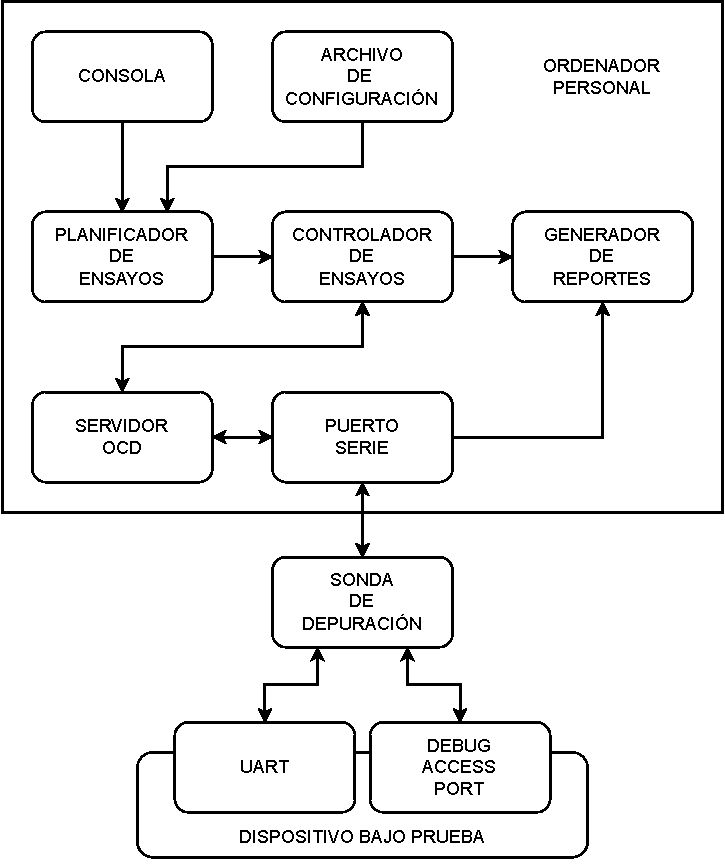
\includegraphics[width=\textwidth]{./Figures/siseblocks.pdf}
    \caption{Diagrama en bloques del sistema de inyección de soft-errors.}
	\label{fig:siseblocks}
\end{figure}

\begin{figure}[htbp]
	\centering
	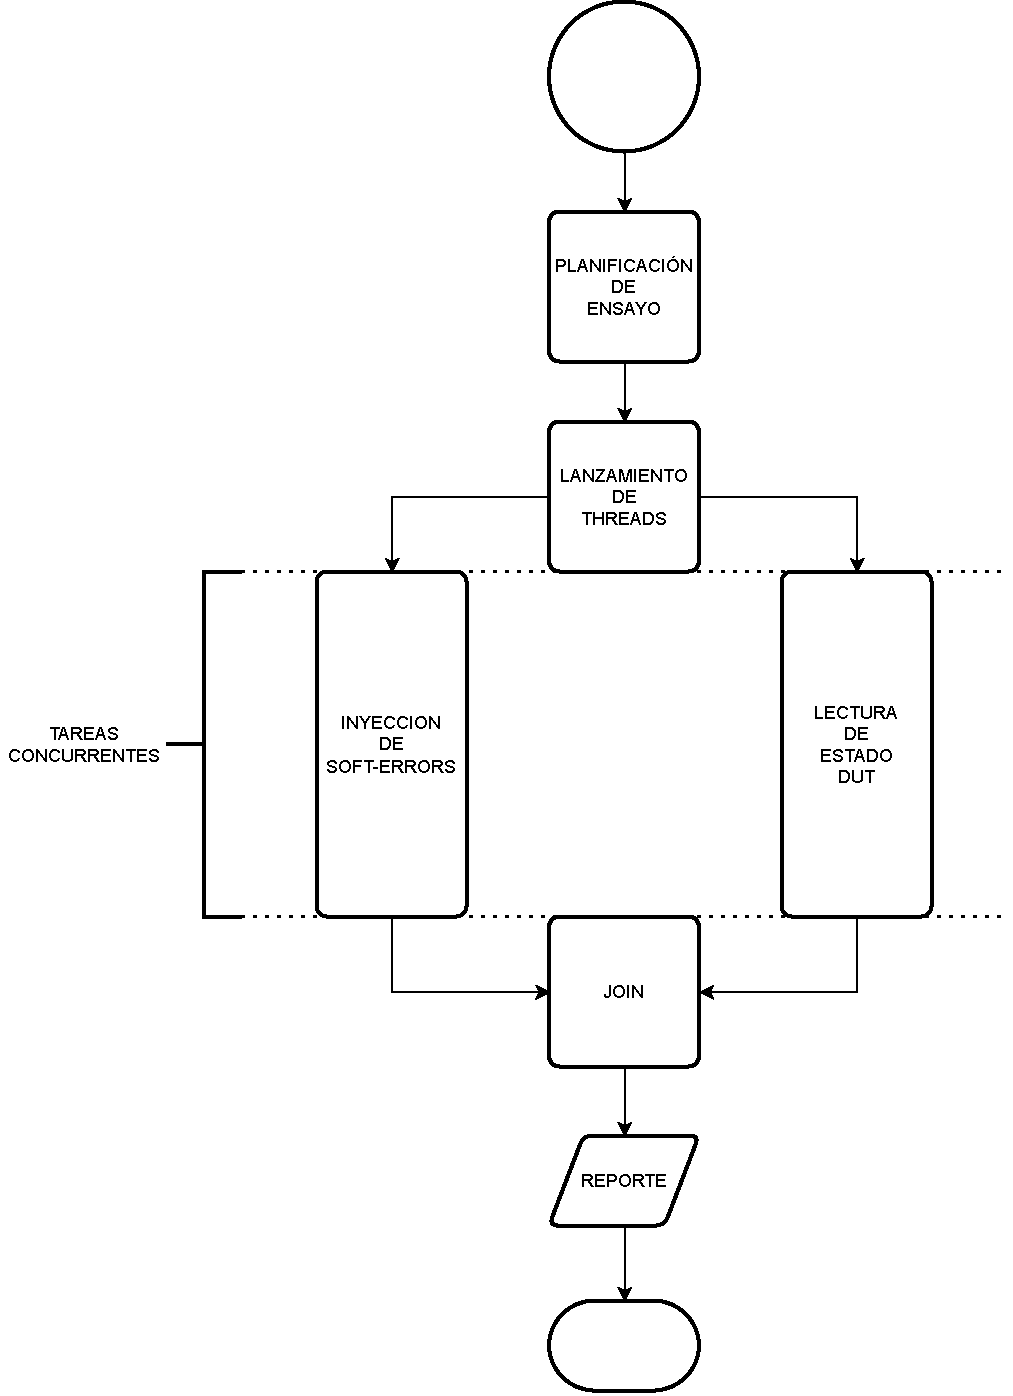
\includegraphics[width=\textwidth]{./Figures/concurrencia.pdf}
    \caption{Flujo de tareas concurrentes.}
	\label{fig:concurrencia}
\end{figure}

\section{Biblioteca para el desarrollo de ensayos}
\label{fig:biblioteca}

Para que el usuario pueda realizar sus propios ensayos, se creó una biblioteca que le provee la funcionalidad necesaria.
Esta biblioteca se divide en dos partes:

\begin{itemize}
    \item Funcionalidades del núcleo.
    \item Funcionalidades de la memoria.
\end{itemize}

Para facilitar la interacción con el núcleo, se implementó una lista con los nombres de los registros.
De esta manera, se facilita el uso de las funciones.
En el código \ref{cod:corereg} se puede observar la colección que se le ofrece al diseñador.

\begin{lstlisting}[language=Python,label=cod:corereg,caption=Lista de registros accesibles por el usuario.]  % Start your code-block

CORE_REGISTERS = [
    'lr', 'pc', 'sp', 'xpsr', 'r0', 'r1', 'r2', 'r3',
    'r4', 'r5', 'r6', 'r7', 'r8', 'r9', 'r10', 'r11', 'r12'
]

\end{lstlisting}

Las funcionalidades ofrecidas para manipular el núcleo del integrado se muestran en el código \ref{cod:coreapi}.
Los detalles son los siguientes:

\begin{itemize}
    \item En la línea 6 se muestra el uso de la función de lectura de registros.
        Se invoca a partir del objeto de conexión y su argumento es el nombre del registro a leer.
    \item En la línea 10 se puede observar el uso del método de escritura de registros.
        Necesita como argumento el nombre del registro y el valor a escribir.
        Luego, la función retorna una tupla con los valores previos y posterior a la escritura.
    \item En la línea 15 se ve una llamada a la función de \emph{bit flip} del registro del núcleo.
        Se debe indicar el nombre del registro y la posición del bit a invertir.
        Finalmente, se retorna el valor previo y posterior al llamado del método.
\end{itemize}


\begin{lstlisting}[language=Python,label=cod:coreapi,caption=Ejemplo de uso en registros del núcleo.]  % Start your code-block

import sise.library as sise

dut = sise.Connection()

# Lectura del registro del CORE
rreg = dut.readRegister('pc')
print("PC:", rreg)

# Escritura del registro del CORE
wreg = writeRegister('r0', 0xffffffff)
print("(old, new):", wreg)

# Bit-flip en registro del CORE
bit = 2
bfreg = bitFlipRegister('r1', bit)
print("(old, new):", bfreg)

del(dut)

\end{lstlisting}

Para interactuar con la memoria se dispone de las funciones demostradas en el código \ref{cod:menapi}.
Los métodos se detallan a continuación:
\begin{itemize}
    \item Línea 7: el método permite realizar una lectura del dato en una posición de memoria.
        El argumento es una dirección alineada de la memoria y el retorno es el valor de una palabra de 32 bits.
    \item Línea 12: esta función se utiliza para escribir una posición alineada de memoria.
        Se necesita pasarle una dirección y un valor a escribir.
        Finalmente, retorna una tupla con el dato previo y posterior a la ejecución del método.
    \item Línea 18: la subrutina posibilita hacer un \emph{bit flip} en una posición de memoria.
        El método toma como argumento una posición alineada de memoria y el bit a invertir.
        Luego de su ejecución, se retorna el valor previo y posterior a la inversión.
\end{itemize}

\begin{lstlisting}[language=Python,label=cod:menapi,caption=Ejemplo de uso en memoria.]  % Start your code-block

import sise.library as sise

dut = sise.Connection()

# Lectura de memoria
addr = 0x20400004
rmen = readMemory(addr)
print("men:", rmen)

# Escritura de memoria
addr = 0x20400008
wmen = writeMemory(addr, 0xfafafafa):
print("(old, new):", wmen)

# Bit-flip en memoria
addr = 0x20400000
bit = 0
bfmen = dut.bitFlipMemory(addr, bit)
print("(old, new):", bfmen)

del(dut)

\end{lstlisting}
